\documentclass[main.tex]{subfiles}


\begin{document}


\subsection{SEARCH-MaP detects long-range RNA--RNA interactions in ribosomal RNA}

We first validated SEARCH-MaP using 16S and 23S ribosomal RNA (rRNA) from \textit{E. coli}.
For each rRNA, we selected two RNA--RNA interactions spanning > [HOW MANY] nt that had been detected in a cell-free system~\cite{Mustoe2019}.
For each interaction, we hypothesized that binding an ASO to either side would break the interaction and perturb the structure of the other side (distant from the ASO binding site) and designed two ASOs, one targeting each side.
As a negative control, we also designed one ASO targeting a stem loop in each rRNA, which we hypothesized would perturb only the structure near the ASO binding site.

We folded the 16S and 23S rRNAs with each ASO, performed DMS-MaPseq over the entire transcripts, and compared ensemble average mutational profiles with and without ASOs using SEISMIC-RNA.
[DESCRIBE THE RESULTS]

\begin{figure}[H]
	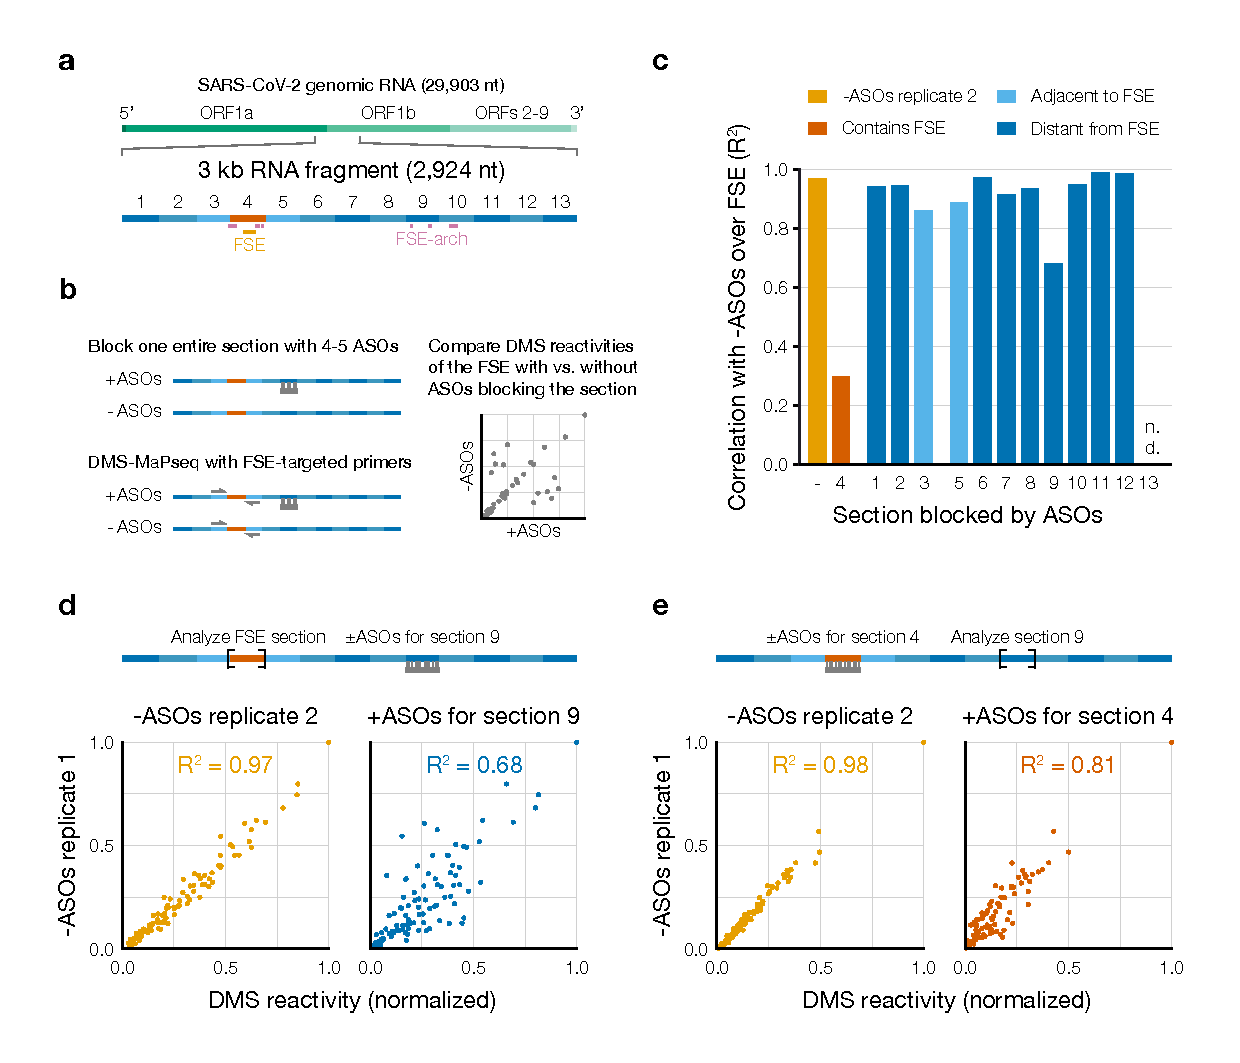
\includegraphics[height=0.95\textheight]{../MainFigures/fig2.pdf}
	\caption{}
	\label{rrna}
\end{figure}


\end{document}
